\documentclass[11pt,letterpaper]{article}
\usepackage[utf8]{inputenc}

%----- Configuración del estilo del documento------%
\usepackage{epsfig,graphicx}
\usepackage[left=2cm,right=2cm,top=1.8cm,bottom=2.3cm]{geometry}
\usepackage{fancyhdr}
\usepackage{lastpage}
\usepackage{url}
\usepackage{tikz}
\pagestyle{fancy}
\fancyhf{}
\fancyhead[R]{\ifnum\value{page}>1 \textbf{\'Algebra Moderna II}\fi}
\rfoot{\textit{Página \thepage}}
%Encabezado izquierdo: logo
\lfoot{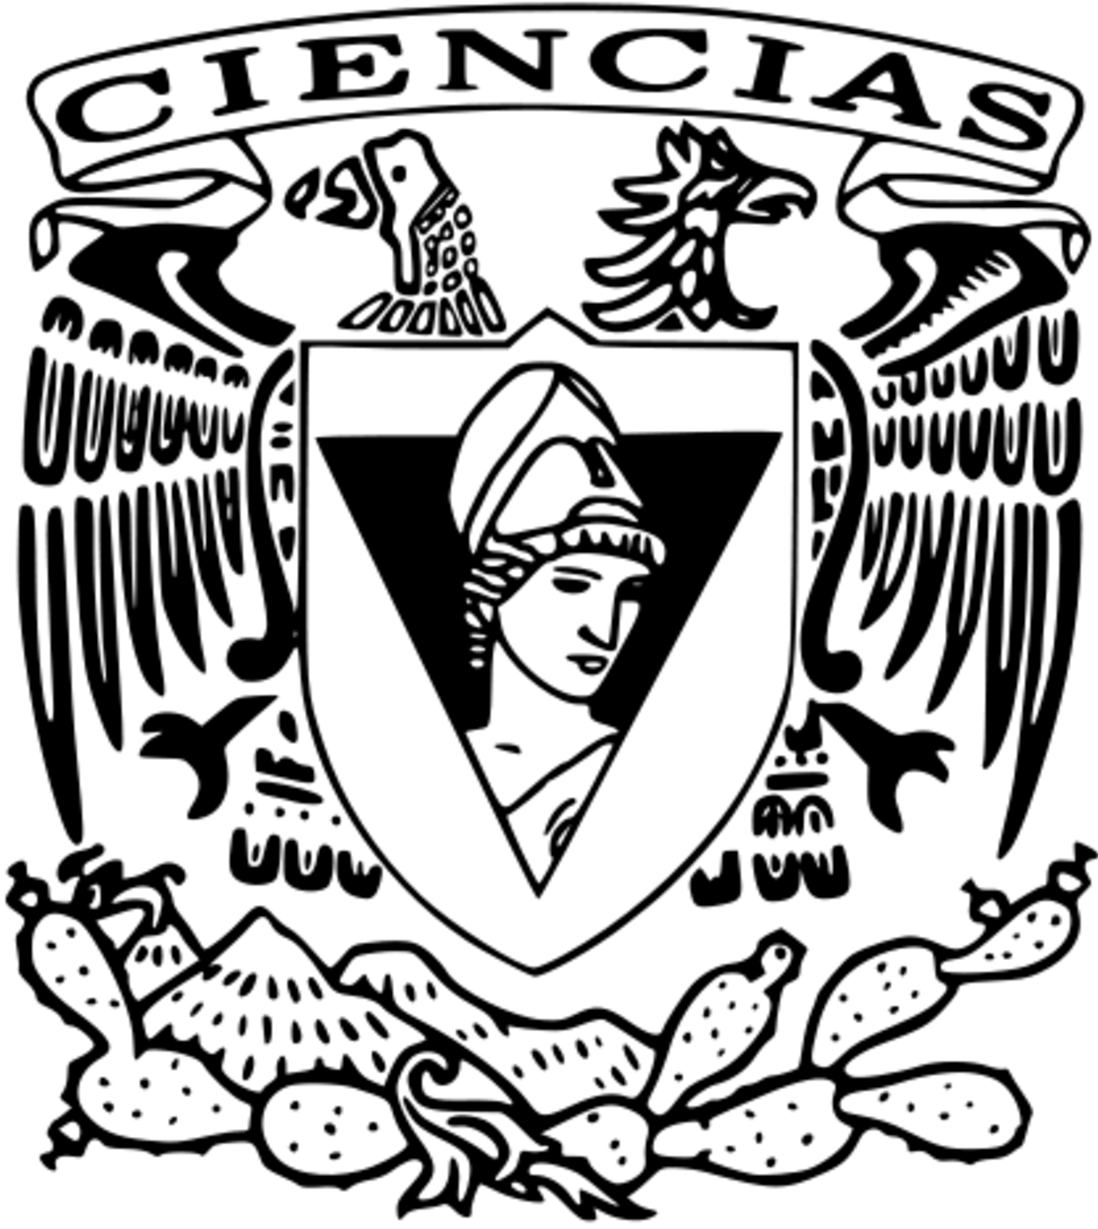
\includegraphics[height=1.0cm]{Logo_FC.png}}
%------ Paquetes matemáticos básicos --------%
\usepackage{amsmath}
\usepackage{amssymb}
\usepackage{amsthm}

\usepackage[spanish]{babel}
\usepackage{graphicx}
\usepackage{hyperref}

\usepackage{tabularx}
\usepackage{xcolor}
\usepackage[table]{xcolor}
\usepackage{colortbl}
\usepackage{array, multirow, multicol, tabularx}
\usepackage{tcolorbox}
\newtheorem{theorem}{Theorem}[section]
\newtheorem{corollary}{Corollary}[theorem]
\newtheorem{lemma}[theorem]{Lemma}

%------si-------%
\definecolor{B}{HTML}{FFFFFF}
\definecolor{G}{HTML}{5e5e5e}
\definecolor{R2}{HTML}{d53d40}
\definecolor{A2}{HTML}{034190}
\definecolor{V2}{HTML}{7faa50}
\newcommand{\R}{\mathbb{R}}
\newcommand{\C}{\mathcal{C}}
\newcommand{\N}{\mathbb{N}}
\newcommand{\Z}{\mathbb{Z}}
\newcommand{\Q}{\mathbb{Q}}
\renewcommand{\theenumi}{\Roman{enumi}}
\renewcommand{\labelenumi}{{\theenumi}.}

\begin{document}
%---Evironment--%
	\makeatletter
        \renewenvironment{proof}[1][\proofname]{\par
            \pushQED{\qed}%
            \normalfont \topsep6\p@\@plus6\p@\relax
            \trivlist
            \item\relax
            {\itshape
            #1\@addpunct{.}}\par\vspace{\baselineskip}\ignorespaces
            }{%
            \popQED\endtrivlist\@endpefalse
            }
        \newenvironment{Solucion}[1][Soluci\'on]{\par
            \pushQED{\qed}%
            \normalfont \topsep6\p@\@plus6\p@\relax
            \trivlist
            \item\relax
            {\itshape
            #1\@addpunct{.}}\par\vspace{\baselineskip}\ignorespaces
            }{%
            \popQED\endtrivlist\@endpefalse
            }
            
    \makeatother

%------ Encabezado -------- %

\begin{center}
    \begin{minipage}{3cm}
    	\begin{center}
    		\includegraphics[height=3.4cm]{logo_unam.png}
    	\end{center}
    \end{minipage}\hfill
    \begin{minipage}{10cm}
    	\begin{center}
    	\textbf{\large Universidad Nacional Autónoma de México}\\[0.1cm]
        \textbf{Facultad de Ciencias}\\[0.1cm]
        \textbf{\'Algebra Moderna 2}\\[0.1cm]
        Tarea examen 2 \\[0.1cm]
         El\'ias L\'opez Rivera\\[0.1cm]
        \texttt{ elias.lopezr,@ciencias.unam.mx }\\[0.1cm]
        Fecha:\,\,5/03/2026
    	\end{center}
    \end{minipage}\hfill
    \begin{minipage}{3cm}
    	\begin{center}
    		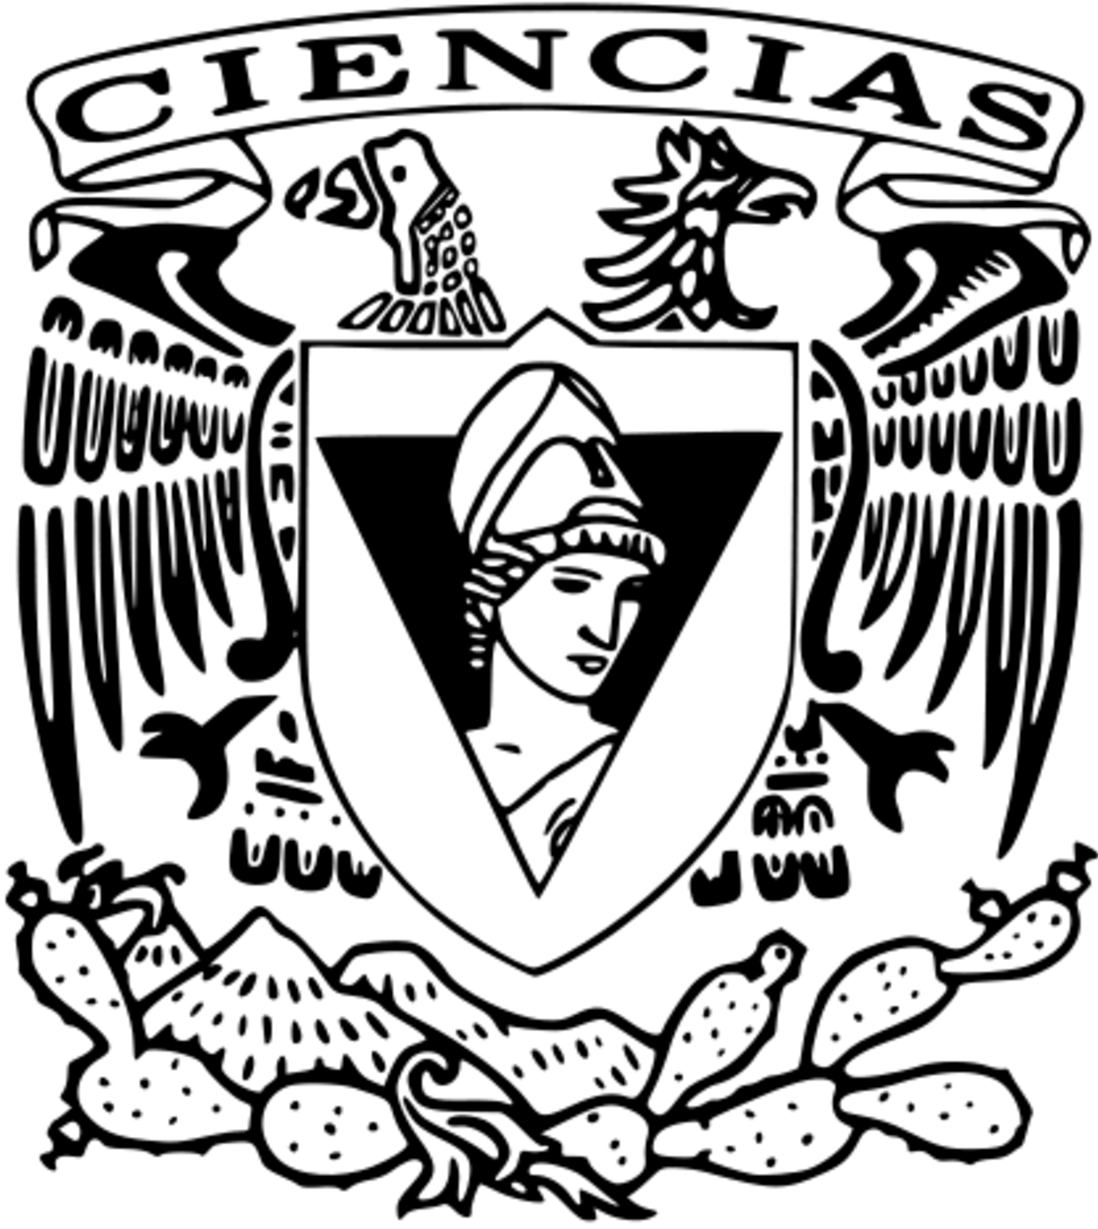
\includegraphics[height=3.4cm]{Logo_FC.png}
    	\end{center}
    \end{minipage}
\end{center}
\rule{17cm}{0.1mm}
%------ Fin de encabezado -------- %
\begin{tcolorbox}[
	title = \textcolor{black}{\textcolor{white}{Problema 1}},]
\textit{Sean $m$ y $n$ enteros positivos primos relativos, utilice el teorema del residuo y los teoremas de isoforfismo para demostrar que
\begin{equation*}
    \Z/ (mn)\Z\equiv\Z/m\Z\times \Z/n\Z
\end{equation*}
Demuestra que $\phi(mn)=\phi(m)\phi(n)$ con $\phi$ la funci\'on de Euler, ademas para $p$ primo $\phi(p^{e})=p^e-p^{e-1}$
Concluya que si $n=\prod_{i=1}^np_i^{e_i}$ con $\{p_i\}_{i\in \N_{n}}$ primos entonces:\,\\
\begin{equation*}
    \phi(n)=\prod_{i}^{n}(p_i^{e_i}-p_i^{e_i-1})=n\prod_{p|n}\left(1-\frac{1}{p_i}\right)
\end{equation*}
}
\end{tcolorbox}
\begin{proof}
    Como $(m,n)=1$, por bezout existe $a,b\in \Z$ tales que $am+bn=1$, por tanto para todo $z\in \Z$, $m(az)=n(bz)=z$, con $m(az)\in m\Z$ y $n(bz)\in n\Z$ por tanto $m\Z$y $n\Z$ son ideales coprimos de $\Z$ aplicando
    el teorema chino del residuo tenemos que $\Z/ (mn)\Z\equiv\Z/m\Z\times \Z/n\Z$\,\\
    \,\\
    Ahora notemos que sea $f:I\to R$ un isomorfismo de anillos, entonces $f$ manda unidades en unidades, pues si $u\in I$ es unidad, existe $v\in I$ tal que
    $uv=1\implies 1=f(uv)=f(u)f(v)$, por tanto podemos resstringir $f$ a $I^{*}$ las unidades de $u$ y obtendremos un isomorfismo de grupos (respecto al producto) entre $I^*$ e $R^*$\,\\
    \,\\
    Finalmente:\,\\
    \begin{equation*}
        \phi(mn)=|(\Z/mn\Z)^*|=|(\Z/m\Z)^*\times (\Z/n\Z)^*|=|(\Z/m\Z)^*||(\Z/n\Z)^*|=\phi(m)\phi(n)
    \end{equation*}\,\\
    Notemos que para $p^{e}$ con $p$ primo sus unicos divisores seran $\{p,2p,\cdots,p^{k-1}(p)\}$ por tanto la cantidad de coprimos sera igual a $p^{e}-p^{e-1}$ es decir $\phi(p^e)=p^{e}-p^{e-1}$, finalmente, podemos
    argumentar por inducci\'on que si $(m_i,m_j)=1$ para todo $i\neq j$ para una lista $S=\{m_i\}_{i\in \N_n}\subset \Z$, entonces $\phi(\prod_{i=1}^n m_i)=\prod_{i=1}^n m_1$, sea $n\in \Z$ por TFA
    existen $\{p_i^{e_i}\}_{i\in \N_k}$ primos tales que $n=\prod_{i=1}^{k}p_i^{e_i}$, como $(p_i^{e-i},p_j^{e_j})=1$ si $i\neq j$ podemos separar:\,\\
    \begin{equation*}
        \phi(n)=\prod_{i=1}^{n}\phi(p_1^{e_i})=\prod_{i=1}^{n}p_1^{e_i}\left(1-\frac{1}{p_1^{e_i}}\right)=n\prod_{p|n}\left(1-\frac{1}{p_i}\right)
    \end{equation*}
\end{proof}\,\\
\begin{tcolorbox}[
	title = \textcolor{black}{\textcolor{white}{Problema 2}},]
\textit{Demuestra que el \'unico homomorfismo de anillos con identidad $\phi:\R\to \R$ es la identidad
}
\end{tcolorbox}
\begin{proof}
   Sea $\varphi:R\to R$ un homomorfismo de anillos. Como $\varphi$ preserva la unidad,
\[
\varphi(1)=1.
\]
 
Además,
\[
\varphi(0)=\varphi(0+0)=\varphi(0)+\varphi(0),
\]
de donde se sigue que $\varphi(0)=0$.
 
Ahora, si $n\in\mathbb N$, entonces
\[
n=\underbrace{1+\cdots+1}_{n\text{ veces}}.
\]
Por homomorfismo,
\[
\varphi(n)
=\varphi(\underbrace{1+\cdots+1}_{n\text{ veces}})
=\underbrace{\varphi(1)+\cdots+\varphi(1)}_{n\text{ veces}}
=\underbrace{1+\cdots+1}_{n\text{ veces}}
=n.
\]
 
Por tanto, $\varphi(n)=n$ para todo $n\in\mathbb N$, es decir, $\varphi$ deja fijos los números naturales, podemos extender esta caracterizaci\'on a $\Z$ pues si $-n\in \Z\implies n\in \N$ y $\phi(-n)=-\phi(n)=n$, ahora sea $m\in \Z$ tenemos
que $m\phi\left(\frac{1}{m}\right)=\phi(m)\phi\left(\frac{1}{m}\right)=\phi(1)=1$ por tanto $\phi\left(\frac{1}{m}\right)=\frac{1}{m}$, por tanto para $\frac{m}{n}\in \Q$ se tiene que $\phi\left(\frac{m}{n}\right)=\frac{m}{n}$.\,\\
\,\\
Ahora notemos que para $x>0$ entonces $x=\sqrt{x}^2$ por tanto $\phi(x)=\phi(\sqrt{x})^2>0$, por tanto si $a<b\implies a-b>0\implies \phi(a-b)=\phi(a)-\phi(b)>0\implies \phi(a)>\phi(b)$, es decir $\phi$ preserva el orden,
ahora para $r\in \R\setminus \Q$ supongamos que $r\neq \phi(r)$ sin perdida de generalidad $\phi(r)<r$ (el caso $r<\phi(r)$ es analogo) por la densidad en $\Q$ existe $m\in\Q$ tal que $\phi(r)<m<r$, como $m<r\implies\phi(m)<\phi(r)$ por tanto $\pi(m)<\phi(r)<\phi(m)$ una contradicci\'on
concluimos que $\phi(r)=r$
\end{proof}\,\\

\begin{tcolorbox}[
	title = \textcolor{black}{\textcolor{white}{Problema 3}},]
\textit{Sea $R$ un anillo con identidad, use el teorema de correspondencia para demostrar que $I$ es m\'aximo $\iff$ $R\backslash I$ es campo
}
\end{tcolorbox}
\begin{proof}
    $\Rightarrow$\,Sea $I\subset R$ un ideal m\'aximo, los unicos ideales que contienen a $I$ son $R$ e $I$, por tanto los \'unicos idelaes de $R/ I$ son $\pi(I)=I/ I=\{0+I\}, \pi(R)=R/ I$, como los unicos ideales
    de $R/ I$ son los triviales $R/ I$ es campo\,\\
    \,\\
    $\Leftarrow$\,\,SI $R\backslash I$ es campo sus unicos ideales son los triviales, de nuevo por teorema de correspondecia los \'unicos dos ideales que contienen a $I$ serian $\pi^{-1}(0+I)=I,\pi^{-1}(R/ I)=R$, por tanto $I$ es m\'aximo
\end{proof}\,\\

\begin{tcolorbox}[
	title = \textcolor{black}{\textcolor{white}{Problema 4}},]
\textit{Sea $R$ un anillo conmutativo con identidad, demuestra que todo ideal m\'aximo de $R$ es primo
}
\end{tcolorbox}
\begin{proof}
    Sabemos  que $I\subset R$ ideal de $R$ es primo si y solo si $R/ I$ es dominio entero, por el problema anterior si $I$ es ideal m\'aximo
    entonces $R/ I$ es campo, todo campo es dominio entero, por tanto $I$ es ideal primo
\end{proof}\,\\
    \begin{tcolorbox}[
	title = \textcolor{black}{\textcolor{white}{Problema 5}},]
\textit{Considere el conjunto:\,\\
\begin{equation*}
    I=\left\{f(x)=\displaystyle\sum_{k=0}^{n}a_kx^k\in \Z[x]:\sum_{k\geq 0, k\,\,par}a_k-\sum_{k\geq 0\,\,k\,\,impar}a_k=0\right\}
\end{equation*}
Demuestra que $I$ es un ideal primo de $\Z[x]$, pero no m\'aximo
}
\end{tcolorbox}
\begin{proof}
    Consideramos el morfimo $Ev_{-1}:\Z[x]\to\Z$ dado por $Ev_{-1}(F(x))=F(-1)$, claramente $ker(Ev_1)=I$, ademas este morfismo es suprayectivo, pues
    para $z\in\Z$ consideramos el polinomio constante $F_{z}(x)=z$, claramente $Ev_{-1}(F_{z}(x))=z$, por primer teorema de isomorfismo $R/I\sim Im(ev_{-1})=\Z$, como $\Z$ es 
    es dominio entero, tenemos que $I$ es ideal primo, notemos que $\Z$ no es campo por tanto $I$ no puede ser ideal m\'aximo
\end{proof}
\begin{tcolorbox}[
	title = \textcolor{black}{\textcolor{white}{Problema 6}},]
\textit{Considere el conjunto:\,\\
\begin{equation*}
    I=\left\{f(x)=\displaystyle\sum_{k=0}^{n}a_kx^k\in \R[x]:\sum_{k\geq 0, k\,\,par}\frac{a_k}{2^k}-\sum_{k\geq 0\,\,k\,\,impar}\frac{a_k}{2^k}=0\right\}
\end{equation*}
Demuestra que $I$ es un ideal m\'aximo de $\R[x]$
}
\end{tcolorbox}
\begin{proof}
    Consideramos el morfimo $Ev_{-1}:\R[x]\to\R$ dado por $Ev_{-1}(F(x))=F(-1)$, claramente $ker(Ev_1)=I$, ademas este morfismo es suprayectivo, pues
    para $r\in\R$ consideramos el polinomio constante $F_{r}(x)=r$, claramente $Ev_{-1}(F_{r}(x))=r$, por primer teorema de isomorfismo $R/I\sim Im(ev_{-1})=\R$, como $\R$ es 
    campo, tenemos que $I$ es ideal m\'aximo
\end{proof}
\begin{tcolorbox}[
	title = \textcolor{black}{\textcolor{white}{Problema 7}},]
\textit{Sean $R$ y $S$ anillos $n\geq 1$.Considere un homomorfismo de anillos:\,\\
\begin{equation*}
    \phi:M_n(R)\to S
\end{equation*}
Demuestra que existe un ideal $I$ de $R$ tal que $im(\phi)\sim M_n(R/ I)$}
\end{tcolorbox}
\begin{proof}
   Por primer teorema de isomorfimo $Ker(\phi)=A\subset M_n(I)$, por tanto existe $I\subset R$ ideal tal que $M_n(R)=A$, es decir $M_n(R)/ M_n(I)$, si tomamos la proyecci\'on canonica $\pi:R\to R/ I$ extendiendola componente por
   componente obtenemos que $im(\phi)\equiv M_n(R)/ M_n(I)\equiv M_n(R/ I)$
\end{proof}
\end{document}